%iffalse
\let\negmedspace\undefined
\let\negthickspace\undefined
\documentclass[journal,12pt,onecolumn]{IEEEtran}
\usepackage{cite}
\usepackage{amsmath,amssymb,amsfonts,amsthm}
\usepackage{algorithmic}
\usepackage{graphicx}
\usepackage{textcomp}
\usepackage{xcolor}
\usepackage{txfonts}
\usepackage{listings}
\usepackage{enumitem}
\usepackage{mathtools}
\usepackage{gensymb}
\usepackage{comment}
\usepackage[breaklinks=true]{hyperref}
\usepackage{tkz-euclide} 
\usepackage{listings}
\usepackage{gvv}                                        
\def\inputGnumericTable{}                                 
\usepackage[latin1]{inputenc}                                
\usepackage{color}                                            
\usepackage{array}                                             
\usepackage{longtable}                                       
\usepackage{calc}                                             
\usepackage{multirow}                                         
\usepackage{hhline}                                           
\usepackage{ifthen}                                           
\usepackage{lscape}
\usepackage{multicol}

\newtheorem{theorem}{Theorem}[section]
\newtheorem{problem}{Problem}
\newtheorem{proposition}{Proposition}[section]
\newtheorem{lemma}{Lemma}[section]
\newtheorem{corollary}[theorem]{Corollary}
\newtheorem{example}{Example}[section]
\newtheorem{definition}[problem]{Definition}
\newcommand{\BEQA}{\begin{eqnarray}}
\newcommand{\EEQA}{\end{eqnarray}}
\newcommand{\define}{\stackrel{\triangle}{=}}
\theoremstyle{remark}
\newtheorem{rem}{Remark}
\begin{document}

\bibliographystyle{IEEEtran}
\vspace{3cm}

\title{NCERT -10.3.4.2.2}
\author{EE224BTECH11044 - Muthyala koushik
}
\maketitle
\bigskip

\renewcommand{\thefigure}{\theenumi}
\renewcommand{\thetable}{\theenumi}
\textbf{\section{DIFFERENTIAL EQUATIONS}}

\textbf{Question:}Five years ago, Nuri was thrice as old as Sonu. Ten years later, Nuri will be twice as old as Sonu. How old are Nuri and Sonu? \\ 

\solution Let Nuri's current age is $x$ and Sonu's current age is $y$: 

\begin{itemize}
	\item Five years ago, Nuri was thrice as old as Sonu.
\end{itemize}
\begin{align}
	x-5=3\brak{y-5} \implies x-3y=-10
\end{align}

\begin{itemize}
	\item Ten years later, Nuri will be twice as old as Sonu.
\end{itemize}
\begin{align}
	x+10=2\brak{y+10} \implies x-2y=10
\end{align}
Given Equations:
\begin{align}
	x - 3y &= -10, \\
	x - 2y &= 10.
\end{align}

Eliminate $x$:
\begin{align}
	(x - 2y) - (x - 3y) &= 10 - (-10), \\
	y &= 20.
\end{align}

Substitute $y = 20$ into the first equation:
\begin{align}
	x - 3(20) &= -10, \\
	x - 60 &= -10, \\
	x &= 50.
\end{align}

Final Answer:
\begin{align}
	x = 50, y = 20.
\end{align}

\textbf{Solution using LU Decomposition}\\
The system of equations can be written in matrix form as:
\begin{align}
    \begin{pmatrix}
        1 & -3 \\
        1 & -2
    \end{pmatrix}
    \begin{pmatrix}
        x \\ y
    \end{pmatrix}
    =
    \begin{pmatrix}
        -10 \\ 10
    \end{pmatrix}.
\end{align}

Let:
\begin{align}
    A =
    \begin{pmatrix}
        1 & -3 \\
        1 & -2
    \end{pmatrix},
    \quad
    \mathbf{x} =
    \begin{pmatrix}
        x \\ y
    \end{pmatrix},
    \quad
    \mathbf{b} =
    \begin{pmatrix}
        -10 \\ 10
    \end{pmatrix}.
\end{align}

\textbf{Doolittle's Algorithm:}\\
The LU decomposition splits $A$ into a lower triangular matrix $L$ and an upper triangular matrix $U$ such that:
\begin{align}
    A = LU
\end{align}
Where:
\begin{align}
    L = 
    \begin{pmatrix}
        1 & 0 & 0 & \cdots & 0 \\ 
        L_{21} & 1 & 0 & \cdots & 0 \\ 
        L_{31} & L_{32} & 1 & \cdots & 0 \\ 
        \vdots & \vdots & \vdots & \ddots & 0 \\ 
        L_{n1} & L_{n2} & L_{n3} & \cdots & 1
    \end{pmatrix}, \quad
    U = 
    \begin{pmatrix}
        U_{11} & U_{12} & U_{13} & \cdots & U_{1n} \\ 
        0 & U_{22} & U_{23} & \cdots & U_{2n} \\ 
        0 & 0 & U_{33} & \cdots & U_{3n} \\ 
        \vdots & \vdots & \vdots & \ddots & U_{n-1,n} \\ 
        0 & 0 & 0 & \cdots & U_{nn}
    \end{pmatrix}.
\end{align}

The Doolittle algorithm is computed as follows:

\textbf{Elements of the $U$ Matrix:}  
For each column $j$:
\begin{align}
    U_{ij} &= A_{ij} \quad \text{if } i = 0,\\
    U_{ij} &= A_{ij} - \sum_{k=0}^{i-1} L_{ik} U_{kj} \quad \text{if } i > 0.
\end{align}

\textbf{Elements of the $L$ Matrix:}  
For each row $i$:  
\begin{align}
    L_{ij} &= \frac{A_{ij}}{U_{jj}} \quad \text{if } j = 0, \\  
    L_{ij} &= \frac{A_{ij} - \sum_{k=0}^{j-1} L_{ik} U_{kj}}{U_{jj}} \quad \text{if } j > 0.  
\end{align}

We decompose the matrix $A$ into the product of a lower triangular matrix $L$ and an upper triangular matrix $U$, i.e., $A = LU$.

Let:
\begin{align}
    L =
    \begin{pmatrix}
        1 & 0 \\
        l_{21} & 1
    \end{pmatrix},
    \quad
    U =
    \begin{pmatrix}
        u_{11} & u_{12} \\
        0 & u_{22}
    \end{pmatrix}.
\end{align}

We compute the elements of $L$ and $U$:
\begin{align}
    u_{11} &= a_{11} = 1, \\
    u_{12} &= a_{12} = -3, \\
    l_{21} &= \frac{a_{21}}{u_{11}} = \frac{1}{1} = 1, \\
    u_{22} &= a_{22} - l_{21} u_{12} = -2 - 1 \cdot (-3) = 1.
\end{align}

Thus, the LU decomposition is:
\begin{align}
    L =
    \begin{pmatrix}
        1 & 0 \\
        1 & 1
    \end{pmatrix},
    \quad
    U =
    \begin{pmatrix}
        1 & -3 \\
        0 & 1
    \end{pmatrix}.
\end{align}


First, solve $L \mathbf{y} = \mathbf{b}$ for $\mathbf{y}$:
\begin{align}
    \begin{pmatrix}
        1 & 0 \\
        1 & 1
    \end{pmatrix}
    \begin{pmatrix}
        y_1 \\ y_2
    \end{pmatrix}
    =
    \begin{pmatrix}
        -10 \\ 10
    \end{pmatrix}.
\end{align}

This gives:
\begin{align}
    y_1 &= -10, \\
    y_1 + y_2 &= 10 \implies -10 + y_2 = 10 \implies y_2 = 20.
\end{align}

Thus:
\begin{align}
    \mathbf{y} =
    \begin{pmatrix}
        -10 \\ 20
    \end{pmatrix}.
\end{align}

Next, solve $U \mathbf{x} = \mathbf{y}$ for $\mathbf{x}$:
\begin{align}
    \begin{pmatrix}
        1 & -3 \\
        0 & 1
    \end{pmatrix}
    \begin{pmatrix}
        x \\ y
    \end{pmatrix}
    =
    \begin{pmatrix}
        -10 \\ 20
    \end{pmatrix}.
\end{align}

This gives:
\begin{align}
    y &= 20, \\
    x - 3y &= -10 \implies x - 3(20) = -10 \implies x = 50.
\end{align}

\textbf{Final Answer:}
\begin{align}
    x = 50, \quad y = 20.
\end{align}

So, Nuri is 50 years old and Sonu is 20 years old.

\begin{figure}[h]
	\centering
	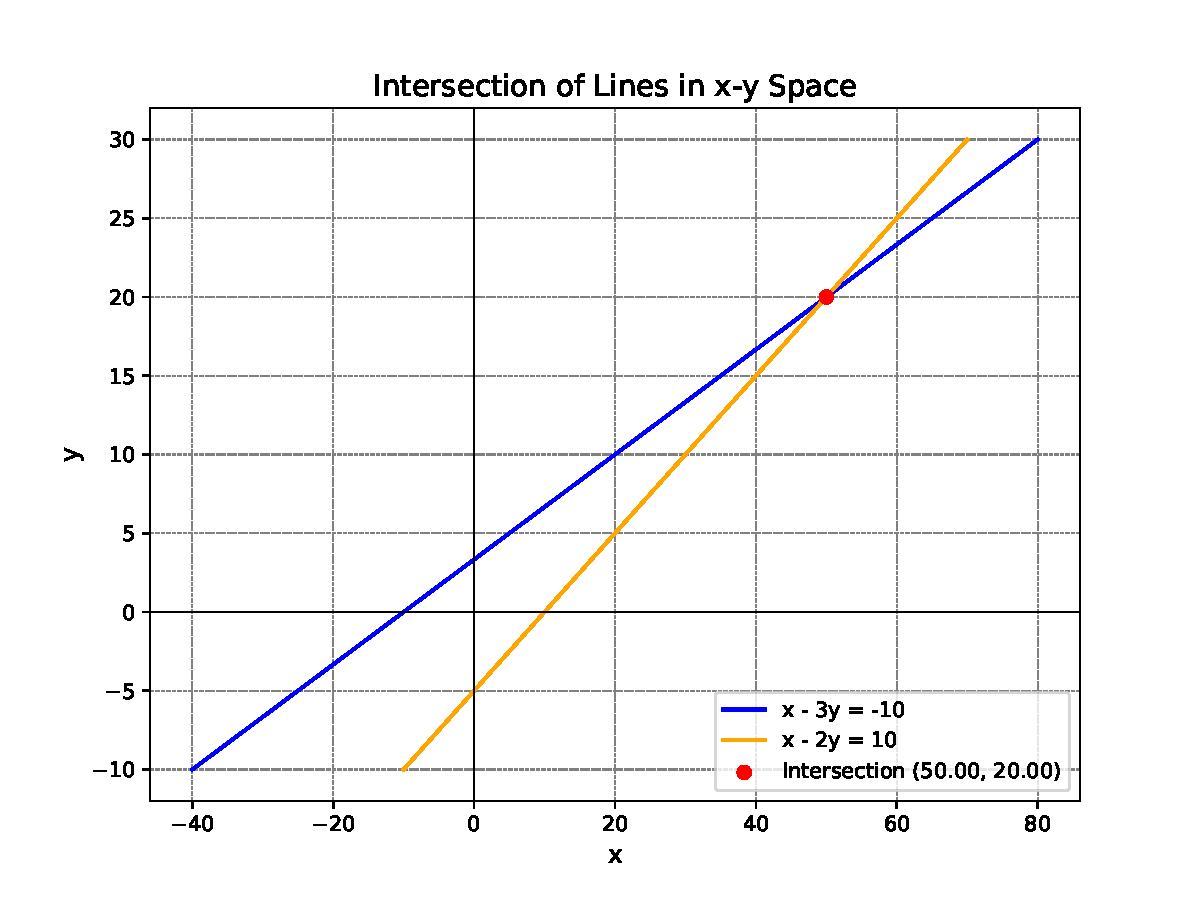
\includegraphics[width=\columnwidth]{figs/fig.pdf}
\end{figure}

\end{document}
